\chapter{Introducción}
\label{chap:intro}

\drop{E}{l} guiado de personas es una actividad que se lleva desarrollando desde siempre con la
ayuda de las estrellas, mapas y brújulas. Afortunadamente para nosotros, desde que se desarrolló
\emph{Transit} en los años sesenta considerado el primer \acf{SGNS} o \acf{GNSS}, resulta
bastante más sencillo conocer nuestra ubicación en el globo de forma precisa y seguir un determinado
camino.

A pesar de que \emph{Transit} se desarrollase en los años sesenta, no fue hasta 1983 cuando
\emph{Honda} se planteó utilizar la tecnología de los \acs{SGNS} para guiar a civiles y desarrolló
su sistema de navegación, culminándolo en 1990 para el \emph{Acura Legend}. Desde entonces se
democratizó el uso de los \acs{SGNS} hasta el punto de encontrar en el mercado un elevado número de
\acf{PDA} equipados con sistemas de navegación a finales de la primera década del 2000.

Con la reciente popularización de los \emph{smartphones} se ha extendido aún más el uso de la
navegación vía satélite y es común encontrar personas utilizándola por medio de aplicaciones como
\emph{Google Maps}, \emph{iOS Maps} o \emph{Nokia HERE}. Como se verá posteriormente, estas
aplicaciones disponen de un gran número de opciones y resultan muy útiles permitiendo llegar
a cualquier sitio sin necesidad de conocer el camino previamente, pero implican un requisito
importante: es necesario ver la pantalla u oír las instrucciones para llevarlas a cabo. Eso no es un
gran inconveniente en un coche, pero para los peatones, ciclistas y motoristas el hecho de mirar a
la pantalla o intentar oír el smartphone supone una distracción que potencialmente puede provocar un
accidente~\cite{Valcarcel12} y, por tanto, para hacer uso de la navegación vía satélite necesitan
otro tipo de interacción con el dispositivo.

Las distracciones del conductor son una de las principales causas de accidentabilidad a nivel
mundial. La \acf{NHTSA} señaló en 2003 que la distracción de los conductores es la causa de 1,5
millones de accidentes producidos anualmente en todo el planeta \cite{RACC03}. Y, según un estudio
de la aseguradora \emph{Allianz} de 2014 \cite{Allianz14}, el 26\% de los accidentes producidos por
distracciones se deben a mirar la pantalla del navegador. Esto hace un total de 390,000 accidentes
que se podrían evitar anualmente cambiando la interacción con el sistema.

Las autoridades de todo el mundo conocen la relación entre distracciones y accidentes e intentan
evitar que se produzcan por medio de su legislación. A día de hoy, en España, el uso de dispositivos
como navegadores, cascos y auriculares por parte del conductor está considerado como una infracción
grave y acarrea una multa de 200 euros y una pérdida de 3 puntos en el carné de conducir
\cite{Serrano14}.

Para hacer frente al problema de las distracciones a la hora de utilizar los sistemas de navegación,
en este trabajo se estudiarán las formas de interacción con el sistema que no supongan una
distracción del usuario. Además se hará un repaso por las diferentes tecnologías, plataformas y
dispositivos sobre los que se puede cimentar un nuevo sistema para conocer las limitaciones técnicas
a las que nos enfrentaremos. Puesto que se trata de un sistema que cambia de estado continuamente
las limitaciones que resultarán significativas están relacionadas con la rapidez y la exactitud de
las tecnologías y dispositivos.

Finalmente, se desarrollará un sistema de guiado en el que el usuario obtendrá realimentación sin
necesidad de ver la pantalla, es decir, por medio de alguna \emph{interacción implícita}. Para ello,
el sistema avisará al usuario en el momento que tenga que realizar cualquiera de las posibles
acciones. La \emph{interacción implícita} que se pretende conseguir con este trabajo se llevará a
cabo por dos medios:

\begin{itemize}
  \item El \textbf{sonido}. Como todos los navegadores actuales nos proporcionará las instrucciones
    de manera auditiva pero como el trabajo va dirigido a peatones, ciclistas y motoristas y resulta
    complicado escuchar nuestro dispositivo en un ambiente abierto, necesitaremos otra interacción
    adicional.
  \item La \textbf{vibración}. Necesaria para las situaciones en las que resulte complicado oír el
    dispositivo y porque está prohibido el uso de cascos o auriculares.
\end{itemize}

Dado el elevado número de posibles instrucciones que el sistema puede comunicar al usuario por medio
de la vibración como giros, cambios de sentido, salidas en una rotonda, etc; será necesario utilizar
más de un dispositivo vibratorio. De esta forma, si se coloca un dispositivo en la parte izquierda
del cuerpo y otro en la parte derecha se pueden codificar de manera inequívoca los giros a la
derecha y a la izquierda haciendo más intuitivas las vibraciones. Esto implica la necesidad de
desarrollar un sistema de comunicaciones entre dispositivos pero se consiguen resultados más
interesantes.

El proyecto pretende utilizar un teléfono (\emph{smartphone}) y su vibrador junto con un periférico
como un reloj (\emph{smartwatch}) o pulsera inteligente (\emph{smartband}). De este modo, cuando
haya que girar a la izquierda vibrará uno, cuando haya que girar a la derecha vibrará el otro y
cuando haya que dar media vuelta vibrarán ambos. De esta manera, si nos colocamos el
\emph{smartwatch} o \emph{smartband} en la mano izquierda y el teléfono en el bolsillo derecho,
cuando tengamos que realizar un giro a la izquierda solamente vibrará el complemento dejando
evidente la acción a realizar (ver Figura~\ref{fig:giroIzquierda}).

\begin{figure}[!h]
  \begin{center}
    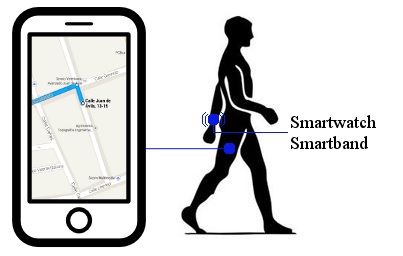
\includegraphics[width=0.65\textwidth]{/esquema-giro-izquierda.png}
    \caption{Ejemplo del sistema indicando un giro a la izquierda}
    \label{fig:giroIzquierda}
  \end{center}
\end{figure}


\section{Estructura del documento}

A continuación se detalla la estructura de este documento para facilitar la lectura del mismo y
se describe brevemente el contenido de cada uno de los capítulos que lo componen.

\begin{definitionlist}
  \item[Capítulo \ref{chap:objetivos}: \nameref{chap:objetivos}] 

  El principal objetivo de este proyecto es el diseño e implementación de un sistema de navegación
  por satélite que se comunique con el usuario por medio de la vibración de alguno de sus
  componentes.

  En este capítulo se detallan los objetivos específicos que se pretenden alcanzar a lo largo
  del desarrollo del proyecto y las limitaciones asociadas.

  \item[Capítulo \ref{chap:antecedentes}: \nameref{chap:antecedentes}]

  En este capítulo se hace una introducción al concepto de \emph{interacción} y sus
  paradigmas. También se hace un repaso de los diferentes sistemas de navegación vía satélite y las
  aplicaciones para \emph{smartphone}. Se pondrá especial interés en la forma que tienen para
  comunicarse con sus usuarios.

  Además, se realizarán estudios que nos permitan realizar buenas elecciones a lo largo del
  \acs{TFG} sobre las plataformas de \emph{smartphones}, los complementos vibratorios y los
  proveedores de mapas y rutas existentes en la actualidad.

  \item[Capítulo \ref{chap:metodo}: \nameref{chap:metodo}]

  El método seleccionado para el desarrollo del trabajo es el \emph{prototipado evolutivo}.

  En este capítulo se describe la metodología seguida, además de especificar las herramientas, tanto
  \emph{hardware} como \emph{software}, utilizadas para la elaboración de este proyecto.

  \item[Capítulo \ref{chap:desarrollo}: \nameref{chap:desarrollo}]

  En este capítulo se encuentra detallado el trabajo realizado especificando cada una de las
  iteraciones necesarias para el desarrollo del proyecto.

  \item[Capítulo \ref{chap:resultados}: \nameref{chap:resultados}]

  En este capítulo se describen los resultados obtenidos tras el desarrollo del sistema y se habla
  sobre los recursos y costes del mismo.

  \item[Capítulo \ref{chap:conclusiones}: \nameref{chap:conclusiones}]

  En este capítulo se detallan las conclusiones obtenidas del desarrollo del proyecto, se
  incluyen posibles usos alternativos del sistema y se proponen posibles líneas de trabajo
  futuras a desarrollar.

\end{definitionlist}

% Local Variables:
%  TeX-master: "main.tex"
%  coding: utf-8
%  mode: latex
%  mode: flyspell
%  ispell-local-dictionary: "castellano8"
% End:
